\chapter{Circulation de fluide dans la cavité trapézoïdale}\label{chap:CircuFluideV2}
\section{Description du modèle}

La cavité située entre la source acoustique principale et le noyau a une forme qui n'est pas conventionnelle, et il est intéressant de développer préalablement un modèle avec une configuration déjà étudiée dans la littérature. En particulier, la convection dans des cavités cylindriques~\cite{schneider_laminar_1992}, ou dans les cavités trapézoïdales~\cite{basak_heat_2009}, doit être étudiée pour donner un aperçu de la forme de la convection naturelle dans le système à l'essai, qui combine ces deux formes.\medskip

La géométrie de la cavité est similaire à celle dans la machine, à savoir un cône tronqué de diamètre du côté de la source principale $D_{SA1}=\qty{108}{\milli\meter}$, un diamètre du côté du noyau $D_{\sf can}=\qty{149}{\milli\meter}$, et une hauteur $L_{\sf cone}=\qty{3}{\centi\meter}$. Contrairement à la zone entourée en jaune sur la figure~\ref{fig:SchemaGeneralTACOT}, seule la partie conique est considérée ici, en omettant le cylindre qui se trouve entre le \echaf{pavillon} du cône et l'échangeur de chaleur froid.\smallskip

La géométrie de la cavité d'adaptation d'impédance est implémentée au sein d'un modèle \textsc{Comsol} suivant la figure~\ref{fig:Comsol_Geometrie_ConeSeul}, pour simuler le comportement, notamment le déclenchement et l'allure éventuelle de cellules de convection naturelle au cours d'études paramétriques dans lesquelles plusieurs paramètres sont variés. Les orientations pour ces simulations sont choisies avec un gradient de température vertical, positif et négatif, et les paramètres balayés lors de l'étude sont la hauteur du cône et le diamètre du col.\medskip

\begin{figure}[!ht]
	\centering
	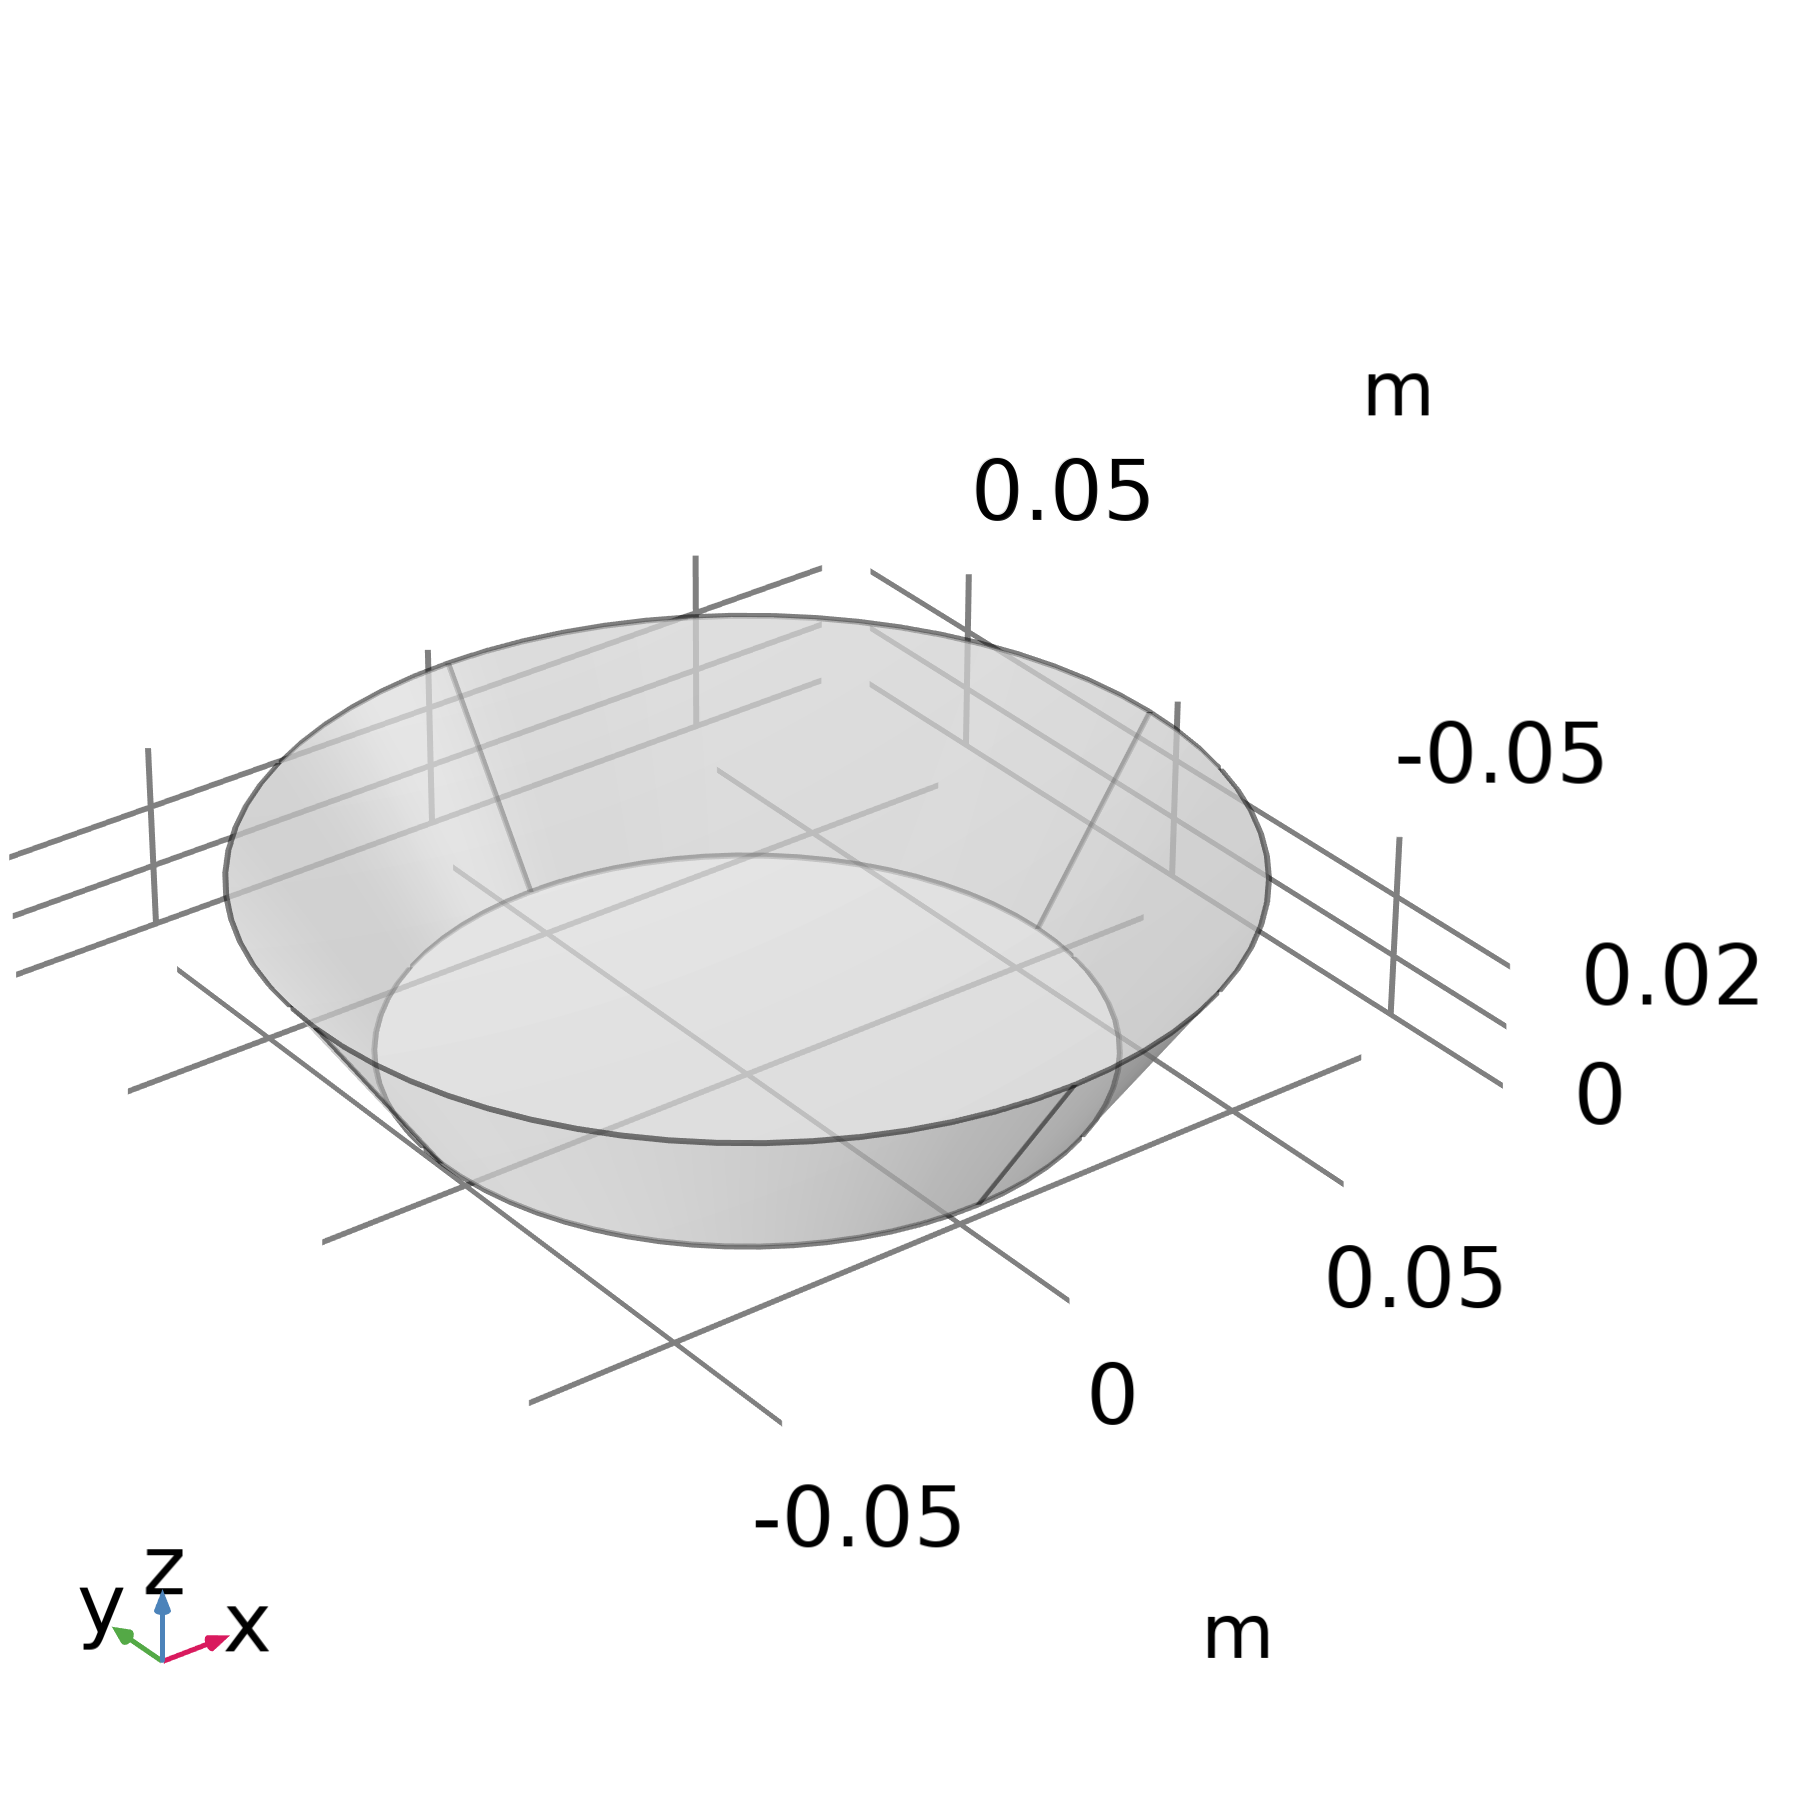
\includegraphics{../fig/fig_ConvNatComsol_Resultats/ConeSeul/Geometrie.png}
	\caption{Géométrie utilisée pour l'étude préliminaire de convection naturelle dans la cavité d'adaptation d'impédance simplifiée.}
	\label{fig:Comsol_Geometrie_ConeSeul}
\end{figure}

Cette cavité est remplie d'hélium à pression atmosphérique, pour comparer avec les résultats du paragraphe~\ref{chap:FEM} pour lequel la pression statique dans la cavité est de \qty{40}{\bar}.\medskip

L'équation de la chaleur est résolue dans le domaine avec l'interface physique \texttt{Heat transfer in Fluids (ht)}, et ce problème est couplé à un modèle d'écoulement \texttt{Laminar flow  (spf)} par l'interface multiphysique \texttt{Nonisothermal flow (nitf)}. L'écoulement est considéré incompressible sous l'approximation de Boussinesq.\smallskip

Les conditions aux frontières pour cette géométrie incluent des parois adiabatiques sur le pourtour du cône, une température $T_c=\qty{293}{\kelvin}$ uniforme sur la section de la paroi haute, et une température $T_f=T_c-\qty{5}{\kelvin}=\qty{288}{\kelvin}$ sur la section de la base du cône. La vitesse est considérée nulle sur toutes les parois.

\section{\'Etude sur la direction du cône}
Dans cette section, le diamètre de la paroi supérieure est gardé constant, et le diamètre de la base du cône $D_{SA1}$ balaye de \qtyrange{54}{97}{\milli\meter}. Trois valeurs sont sélectionnées : la première correspond aux dimensions de la cavité dans le modèle décrit dans le paragraphe~\ref{chap:FEM}, La deuxième valeur du diamètre est celle de la paroi qui lui fait face, de sorte à obtenir un cylindre. La troisième valeur est choisie de manière à avoir le même angle pour le cône, en ayant cette fois le col en haut. Cette dernière configuration est quasi-identique à l'orientation `\texttt{V2}'.\smallskip

Pour chacune de ces géométries, le calcul est effectué, et la composante verticale de la vitesse $v_{0,z}$ est tracée sur la figure~\ref{fig:ConvNatComsol_ConeParamRix}.

\begin{figure}[!ht]
	\centering
	\begin{subfigure}{.97\textwidth}
	\centering
	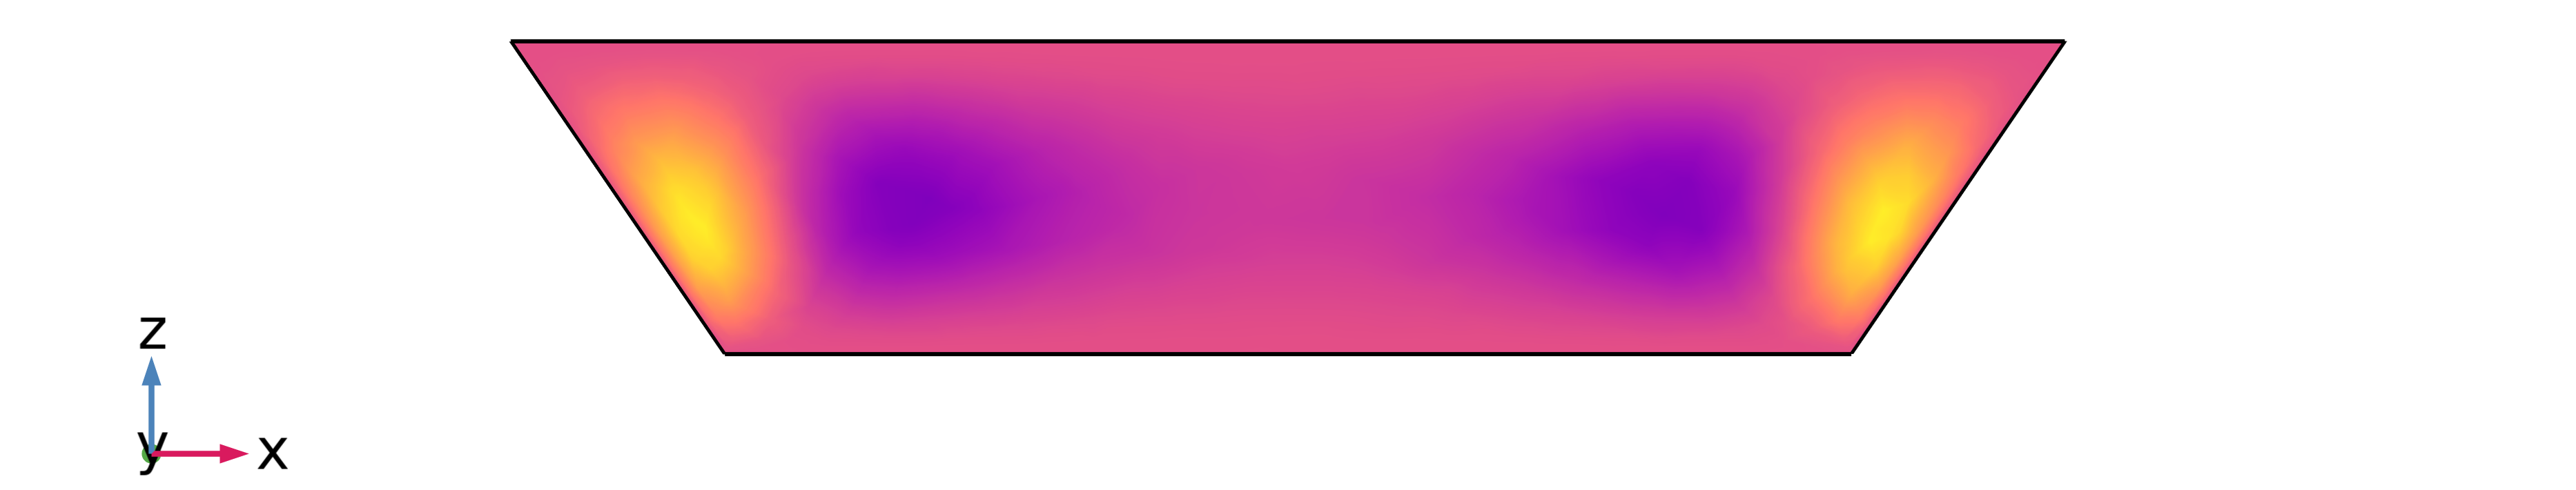
\includegraphics{../fig/fig_ConvNatComsol_Resultats/ConeSeul/SmallBase_THAbove}
	\caption{}
	\label{fig:ConvNatComsol_ConeParamRix_SmallBase}
	\end{subfigure}
	
	\vspace{1em}
	
	\centering
	\begin{subfigure}{.97\textwidth}
	\centering
	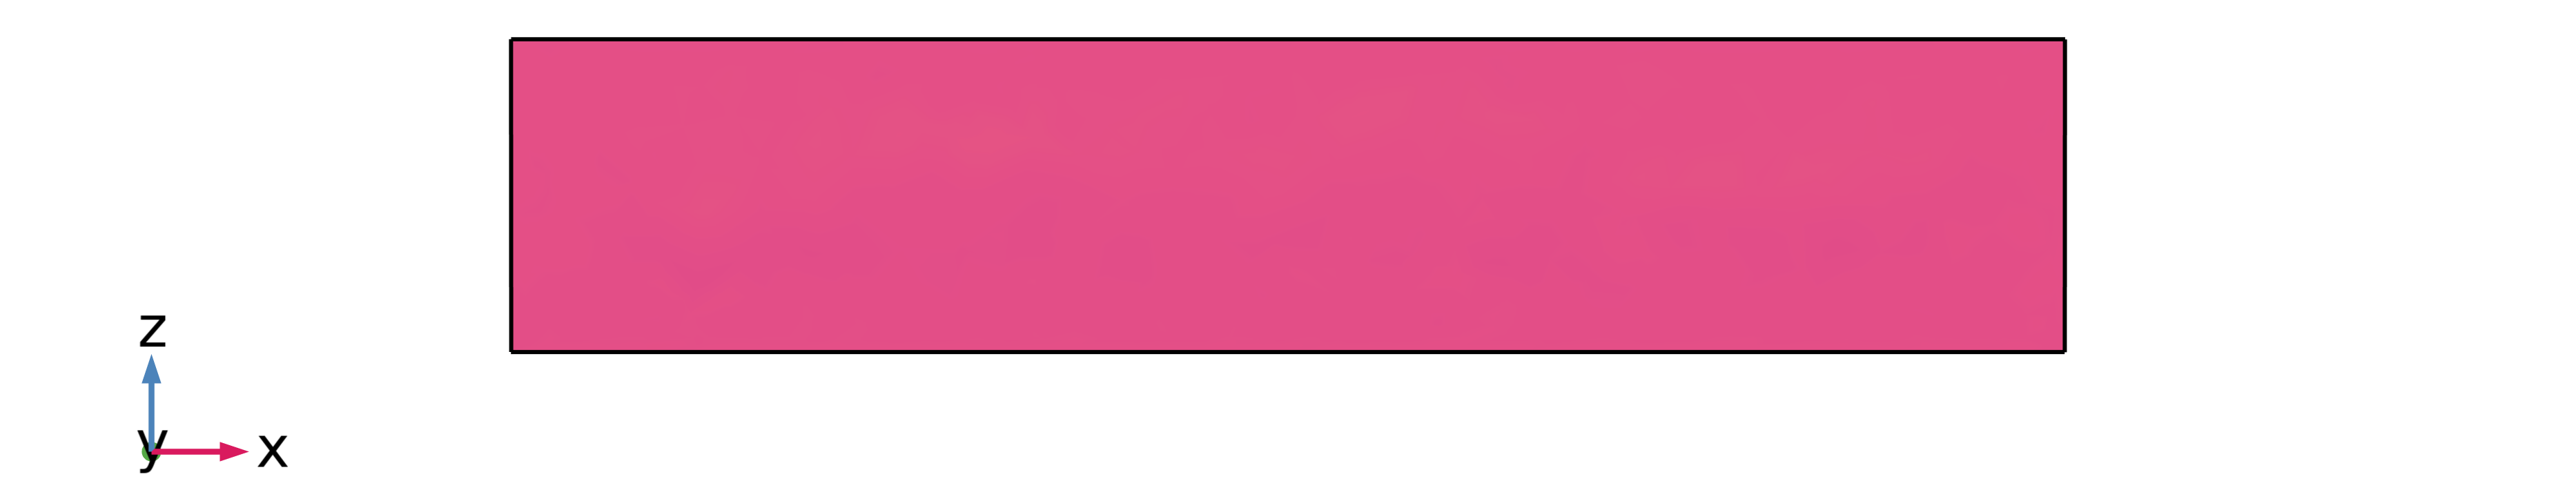
\includegraphics{../fig/fig_ConvNatComsol_Resultats/ConeSeul/Cylinder_THAbove}
	\caption{}
	\label{fig:ConvNatComsol_ConeParamRix_Cylinder}
	\end{subfigure}
	
	\vspace{1em}
	
	\centering
	\begin{subfigure}{.97\textwidth}
	\centering
	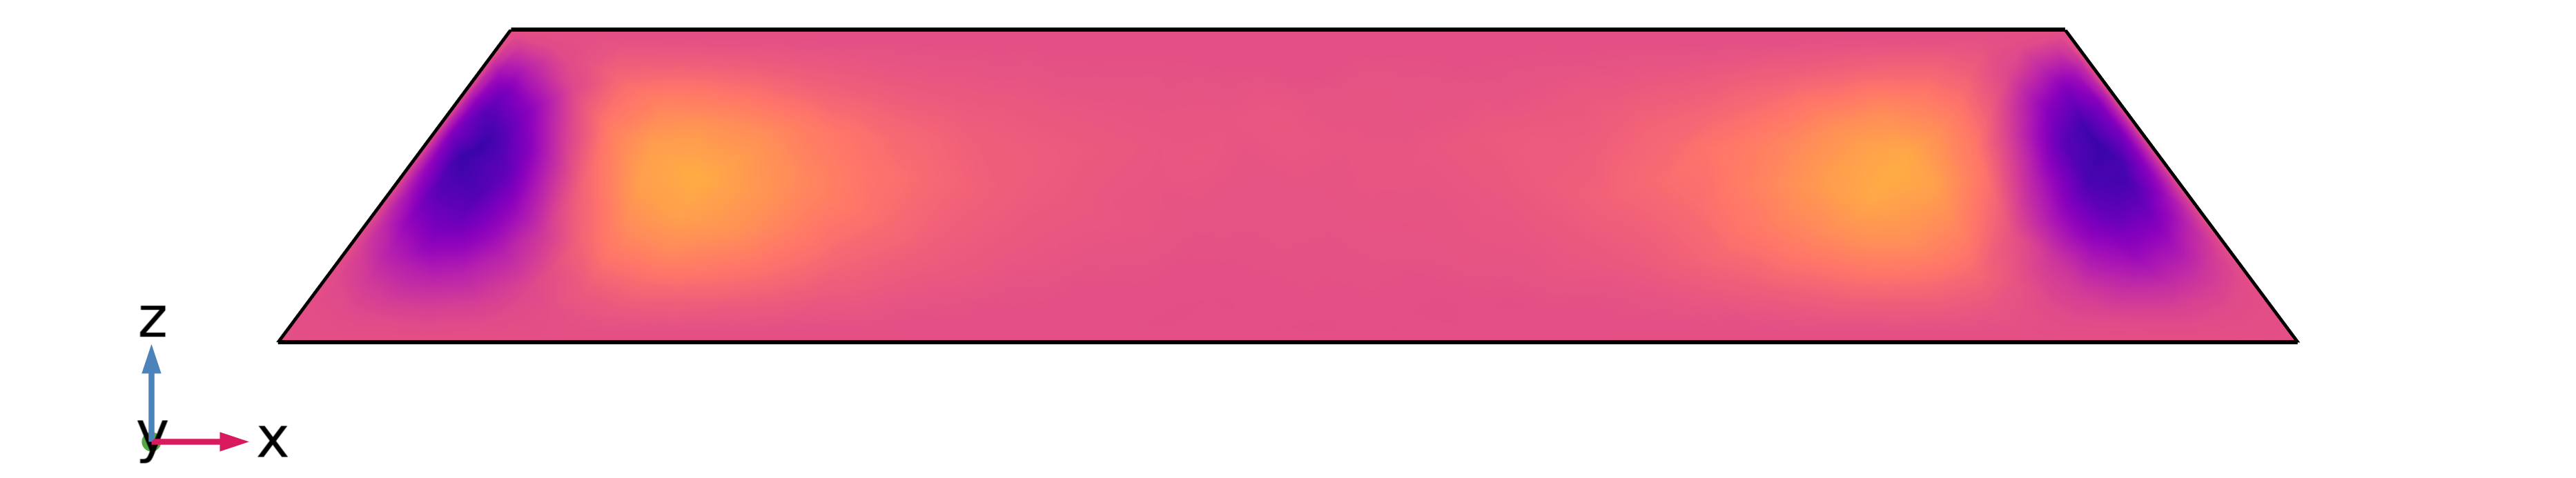
\includegraphics{../fig/fig_ConvNatComsol_Resultats/ConeSeul/LargeBase_THAbove}
	\caption{}
	\label{fig:ConvNatComsol_ConeParamRix_LargeBase}
	\end{subfigure}
	\begin{subfigure}[t]{.47\textwidth}    
      	\centering
		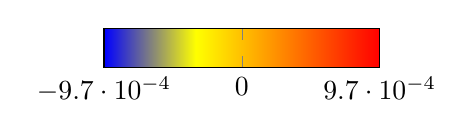
\begin{tikzpicture}[rotate=0]
			\begin{axis}[
		    	hide axis,
            	scale only axis,
           		height=0pt,
                width=0pt,
                colorbar horizontal,
                point meta min=-9.7e-4,
                point meta max=9.7e-4,
                colorbar style={
                	scaled ticks=false, 
%					tick label style={/pgf/number format/fixed},
                	width=3.5cm,
                	xtick={-9.7e-4,0,9.7e-4},
                	at={(-0.5,0.0)},anchor=south,   
                	title style={xshift=3.5cm,yshift=4cm},
                	}
				]
            	\addplot [draw=none] coordinates {(0,0) (1,1)};
        	\end{axis}
		\end{tikzpicture} 
	\end{subfigure} 
	\caption{Composante verticale de la vitesse dans la cavité conique pour trois géométries.}
	\label{fig:ConvNatComsol_ConeParamRix}
\end{figure}

Dans chaque cas, la paroi chaude est en haut de la géométrie, et la paroi froide, en bas. Lorsque la géométrie est conique, la vitesse n'est pas nulle, et une cellule se met en place dans la cavité. Lorsque la paroi de plus petit diamètre est en bas, le fluide monte par la périphérie, et redescend au centre. C'est l'inverse lorsque la paroi de plus petit diamètre est en haut, où le fluide monte par le centre et redescend par les côtés. Lorsque la cavité est cylindrique, la vitesse est nulle, ce qui est le résultat attendu pour cette configuration où il est attendu \textit{a priori} que l'instabilité de Rayleigh-Bénard ne puisse pas apparaître.
